\documentclass[11pt, titlepage]{article}
\usepackage{amsmath,amsthm,amssymb}
\usepackage{hyperref, pgf, tikz}
\usepackage{fancyhdr}
\usetikzlibrary{arrows}
\usepackage[margin=1.25in]{geometry}
\usepackage{graphicx}                     
\pagestyle{fancy}
\usepackage{array}
\usepackage{indentfirst}
%\usepackage{wrapfig}

\lhead{Lab \#6}
\rhead{\thepage}
\cfoot{}

\title{Introduction to the Microwave Optics System and Reflection \\ \ \\ \large Lab \#6}
\author{Name: Avery Karlin \\ Partner: Dalton Wu}
\date{}
\begin{document}

\maketitle

\begin{center}
\LARGE Introduction to the Microwave Optics System and Reflection
\end{center}

\section*{Objective}
The objective of the lab is to measure the time constant of an RC circuit based on an oscilloscope.

\section*{Introduction}
As written about in previous labs, for some charging capacitor in an RC circuit, meaning a circuit with a resistor, a capacitor, and a DC power source, it can be derived that $V = V_0(1 - e^{\frac{-t}{RC}}) = V_0(1 - e^{\frac{-t}{\tau}})$, where $\tau = RC$, signifying the time constant for the RC circuit. Since exponential functions must take a unitless input, the time constant as a result must also have a unit of seconds. As a result, we can say that when $t = \tau$, $V = V_0(1 - e^{-1}) = V_0(0.63)$, such that at that point, the voltage is equal to 63\% of the maximum voltage it will achieve. Similarly, the discharging is described by the equation $V = V_0e^{\frac{-t}{RC}} = V_0e^{\frac{-t}{\tau}}$.

In an AC circuit, on the other hand, there does not need to be a cyclical current flow, due to it being unable to travel infinitely, but rather reversing itself after a brief period of time, discharging the capacitor again, such that it can be connected in series, creating alternating charging and discharging. As a result though, the time it takes to reach 63\% of the maximum height can be found as tau.

\section*{Procedures and Results}

First, the scale of voltage per division must be set such that the total graph moves through 8 divisions vertically, with the frequency generator set to some constant frequency in a square wave pattern, such that the voltage is alternating but not varying, and such that 5 divisions is approximately 63\% of the total height. After, the circuit is set up fully in series, without an ending connection from the oscilloscope back to the AC. The variable resistor and capacitor are then set to some value, measuring the number of horizontal divisions to move up 5 vertical, then repeating for two different resistances and one other capacitance. 

\begin{figure}[h]
\centering
\hspace*{0cm}
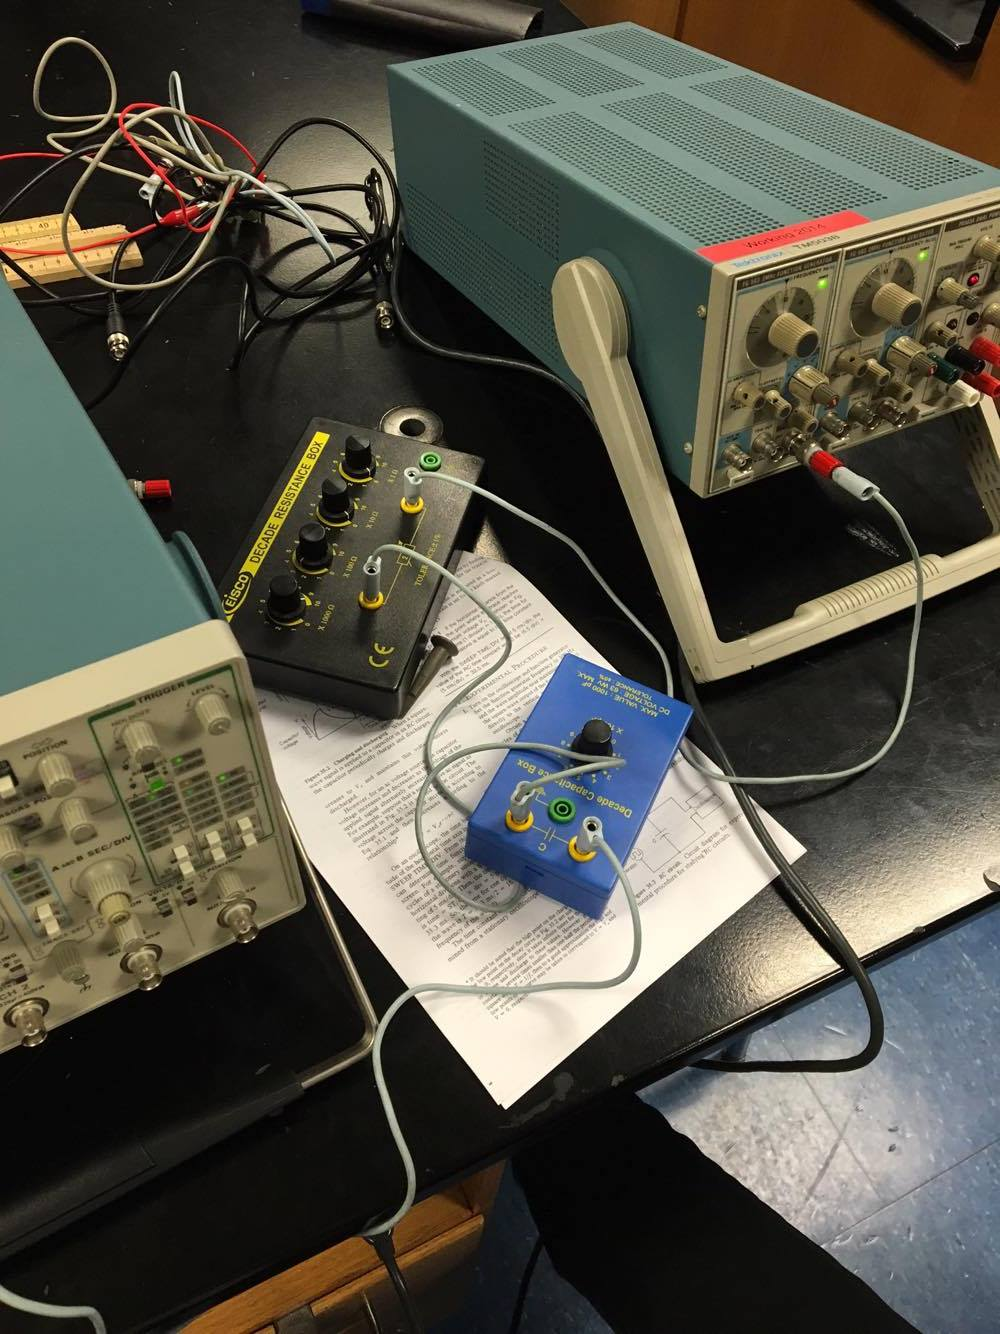
\includegraphics[scale=0.4]{lab51.jpg}
\vspace*{0cm}
\end{figure}

\begin{figure}[h]
\centering
\hspace*{0cm}
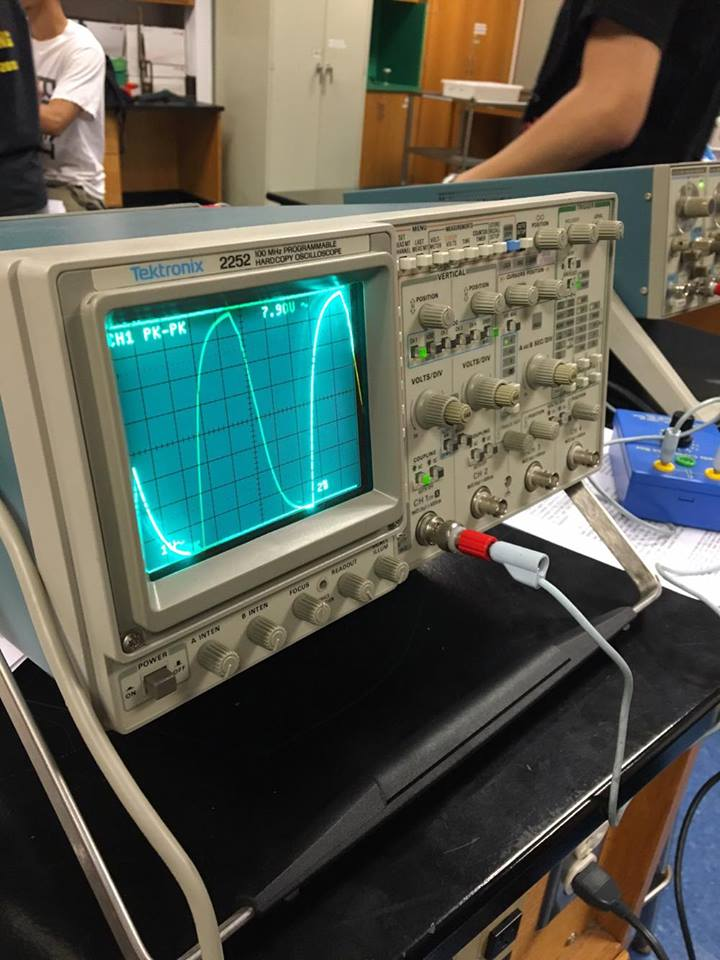
\includegraphics[scale=0.6]{lab52.jpg}
\vspace*{0cm}
\end{figure}

\underline{Resistance Change:}
\begin{center}
$$C = 1 nF$$
\begin{tabular}
{|m{7em}|m{7em}|m{7em}|m{7em}|}
\hline
Trial & Resistance ($\Omega$) & Divisions per 0.63 Rise & Sweep Time/Div (ms/div)\\
\hline
1 & 10k & 2.1 & 2\\
\hline
2 & 5k & 2.1 & 2\\
\hline
3 & 3k & 2.1 & 2\\
\hline
\end{tabular}
\end{center}

\underline{Capacitance Change:}
\begin{center}
$$R = 10 k\Omega$$
\begin{tabular}
{|m{7em}|m{7em}|m{7em}|m{7em}|}
\hline
Trial & Capacitance (pF) & Divisions per 0.63 Rise & Sweep Time/Div (ms/div)\\
\hline
1 & 700 & 2.7 & 2\\
\hline
2 & 400 & 1.2 & 2\\
\hline
\end{tabular}
\end{center}

\section*{Discussion}
Sample calculations for the non-measured data are as shown using the formulas found above:

$$RC_{exp} \text{(Trial 1, Resistance)} = \text{Divisions per 0.63 rise} * \text{Sweep Time per Div} = 2.1 * 2 = 4.2 ms$$
$$RC_{calc} \text{(Trial 1, Resistance)} = R * C = 10k \Omega * 1 nF = 10 ms$$
$$\text{Percent Error (Trial 1, Resistance)} = \frac{\text{$|$Expected - Actual$|$} * 100\%}{\text{Expected}} = \frac{|4.2 - 10| * 100\%}{10} = 58\%$$

\underline{Resistance Change:}
\begin{center}
\begin{tabular}
{|m{7em}|m{7em}|m{7em}|m{7em}|}
\hline
Trial & $RC_{exp}$ (ms) & $RC_{calc}$ (ms)& Percent Error\\
\hline
1 & 4.2 & 10 & 58\\
\hline
2 & 4.2 & 5 & 16\\
\hline
3 & 4.2 & 3 & 40\\
\hline
\end{tabular}
$$\text{Slope of $\tau$ vs R} = 0 F$$
$$\text{Percent Difference of Slope and C} = 100\%$$
\end{center}

\begin{figure}[h]
\centering
\hspace*{0cm}
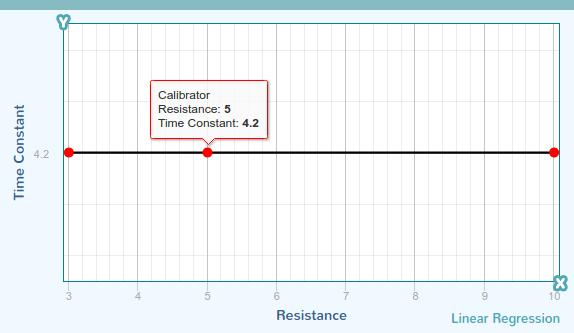
\includegraphics[scale=0.8]{graph51.jpg}
\vspace*{0cm}
\end{figure}

\underline{Capacitance Change:}
\begin{center}
\begin{tabular}
{|m{7em}|m{7em}|m{7em}|m{7em}|}
\hline
Trial & $RC_{exp}$ & $RC_{calc}$ & Percent Error\\
\hline
1 & 5.4 & 7 & 22.9\\
\hline
2 & 2.4 & 4 & 40\\
\hline
\end{tabular}
$$\text{Slope of $\tau$ vs C} = 3000 \Omega$$
$$\text{Percent Difference of Slope and R} = 70\%$$
\end{center}

\begin{figure}[h]
\centering
\hspace*{0cm}
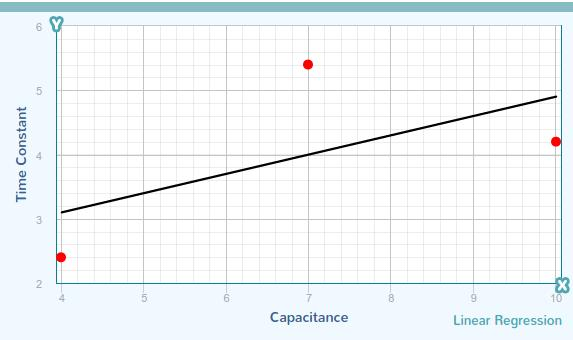
\includegraphics[scale=0.8]{graph52.jpg}
\vspace*{0cm}
\end{figure}

For the change in resistance, the main error seems to be that resistance doesn't impact the time constant experimentally. This is due to the resistance being affected by the frequency, such that the change in resistance for the same frequency has to be far greater to impact the experimental time constant. As a result, for the same frequency and capacitance, within a small region of changes in the resistance, the time constant is the same experimentally for RC circuits. In addition, difficulty operating the oscilloscope itself can account for a portion of the error. In addition, additional resistance due to non ideal wires could bring the experimental time constant up relative to the actual time constant to some degree, though this appears to have had a generally minor effect. 

\section*{Conclusion}

The time constant for the resistance changing trials, for a calculated RC of 10 ms was 4.2 ms with 58\% error, 5 ms was 4.2 ms with 16 \% error, and 3 ms was 4.2 ms with 40\% error. Thus, the slope of $\tau$ vs R was 0 F to the actual capacitance of 1 nF for a percent error of 100\%. The time constant for the capacitance changing trials, for a calculated RC of 7 ms was 5.4 ms with 22.9\% error, and 4 ms was 2.4 ms with 40\% error. Thus, the slope of $\tau$ vs C was 3 $k\Omega$ to the actual resistance of 10 $k\Omega$ for a percent error of 70\%.

\end{document}
